\documentclass{beamer}

\usetheme{Madrid}
\usecolortheme{seahorse}

\usepackage{geometry}
\usepackage{graphicx}
\usepackage{amssymb}
\usepackage{epstopdf}
\usepackage{amsmath}  	% this permits text in eqnarray among other benefits
\usepackage{color}          	% gives color options
\usepackage{url}		% produces hyperlinks
\usepackage[english]{babel}
\usepackage[latin1]{inputenc}
\usepackage{colortbl}	% allows for color usage in tables
\usepackage{multirow}	% allows for rows that span multiple rows in tables
\usepackage{xcolor}		% this package has a variety of color options
\usepackage{calc}
\usepackage{multicol}

\setbeamertemplate{navigation symbols}{}

%User defined colors: See colors section
\xdefinecolor{oiBlue}{rgb}{0.15, 0.35, 0.55}
\xdefinecolor{gray}{rgb}{0.5, 0.5, 0.5}
\xdefinecolor{darkGray}{rgb}{0.3, 0.3, 0.3}
\xdefinecolor{darkerGray}{rgb}{0.2, 0.2, 0.2}
\xdefinecolor{rubineRed}{rgb}{0.89,0,0.30}
\xdefinecolor{linkCol}{rgb}{0.11,0.49,0.95}	
\xdefinecolor{irishGreen}{rgb}{0,0.60,0}	
\xdefinecolor{darkturquoise}{rgb}{0.44, 0.58, 0.86}
\definecolor{lightGreen}{rgb}{0.533,0.765,0.42}

\setbeamercolor*{palette primary}{fg=white,bg= oiBlue!70}
\setbeamercolor*{palette secondary}{fg=black,bg= oiBlue!20!white}
\setbeamercolor*{palette tertiary}{fg=white,bg= oiBlue!80!black!90}
\setbeamercolor*{palette quaternary}{fg=white,bg= oiBlue}

\setbeamercolor{structure}{fg= oiBlue}
\setbeamercolor{frametitle}{bg= oiBlue!70}

\setbeamercolor{disc body}{bg=oiBlue!20!white!80,fg=oiBlue!80!black!90}
\setbeamercolor{disc title}{bg=oiBlue!40!white!60,fg=oiBlue!70!black!100}


\setbeamertemplate{blocks}[shadow=false]


\newcommand{\removepagenumbers}{% 
  \setbeamertemplate{footline}{
    %
    \begin{beamercolorbox}[colsep=1.5pt]{upper separation line foot}
    \end{beamercolorbox}
    \begin{beamercolorbox}[ht=2.5ex,dp=1.125ex,%
      leftskip=.3cm,rightskip=.3cm plus1fil]{author in head/foot}%
      \leavevmode{\usebeamerfont{author in head/foot}\insertshortauthor}%
%      \hfill%
%      {\usebeamerfont{author in head/foot}\usebeamercolor[fg]{institute in head/foot}\insertshortinstitute}%
    \end{beamercolorbox}%
    \begin{beamercolorbox}[ht=2.5ex,dp=1.125ex,%
      leftskip=.3cm,rightskip=.3cm plus1fil]{title in head/foot}%
      {\usebeamerfont{title in head/foot}\insertshorttitle}%
      \hfill%
      {\usebeamerfont{author in head/foot}\usebeamercolor[fg]{institute in head/foot}\insertshortinstitute}%
    \end{beamercolorbox}%
    \begin{beamercolorbox}[colsep=1.5pt]{lower separation line foot}
    \end{beamercolorbox}
    }
} 


\newcommand{\disc}[2]{
\begin{beamerboxesrounded}[shadow = true, lower = disc body, upper = disc title]{#1}
#2
\end{beamerboxesrounded}
}


\AtBeginSection[] 
{ 
  \addtocounter{framenumber}{-1} 
  % 
  {\removepagenumbers 
    \begin{frame}<beamer> 
    \tableofcontents[currentsection] 
  \end{frame} 
  } 
} 

\usepackage{isotope}
\usepackage{bm}
\usepackage{minted}

\newcommand{\pkg}[1]{{\normalfont\fontseries{b}\selectfont #1}} 


\title[UseR! 2013]{Leveraging GPU libraries for efficient computation of Gaussian process models in \textit{R}}
\author{Colin Rundel}
\date{July 10, 2013}
\institute[Duke]{Duke University, Department of Statistical Science}


\begin{document}

\begin{frame}[plain]
\titlepage
\end{frame}

%==================================================================================================
%==================================================================================================

\section{Background}
\addtocounter{framenumber}{-1} 

%==================================================================================================

\begin{frame}
\frametitle{Background}


Using intrinsic markers (genetic and isotopic signals) for the purpose of inferring migratory connectivity.

\begin{itemize}
\item Existing methods are too coarse for most applications
\item Large amounts of data are available ( \textgreater{}150,000 feather samples from \textgreater{}500 species)
\item Genetic assignment methods are based on Wasser, et al. (2004)
\item Isotopic assignment methods are based on Wunder, et al. (2005)
\end{itemize}

\vspace{3mm} \pause

Paper - Rundel, C.W., \textit{et al.} (2013) Novel statistical methods for integrating genetic and stable isotopic data to infer individual-level migratory connectivity. \textit{Molecular Ecology}. (\textit{in press})

\end{frame}


%==================================================================================================

\begin{frame}[t]
\frametitle{Data - DNA microsatellites and $\delta \isotope[2]{H}$}

\begin{columns}[t]
\column{0.5\textwidth}
Hermit Thrush (\textit{Catharus guttatus}) \\
\vspace{2mm}
\begin{itemize}
\item 138 individuals
\item 14 locations
\item 6 loci
\item 9-27 alleles / locus
\end{itemize}
\column{0.5\textwidth}
Wilson's Warbler (\textit{Wilsonia pusilla}) \\

\begin{itemize}
\item 163 individuals
\item 8 locations
\item 9 loci
\item 15-31 alleles / locus
\end{itemize}

\end{columns}

~\\
~\\

\begin{columns}
\column{0.5\textwidth}
\begin{center}
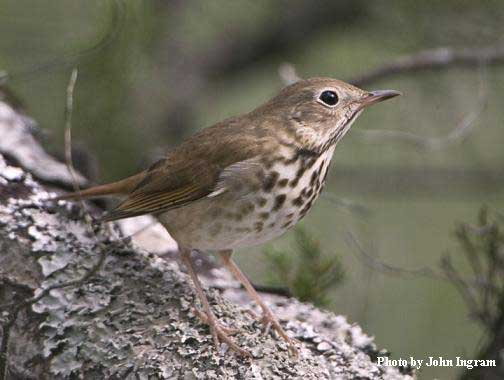
\includegraphics[width=0.65\textwidth]{pics/hermit_thrush.jpeg}
\end{center}
\column{0.5\textwidth}
\begin{center}
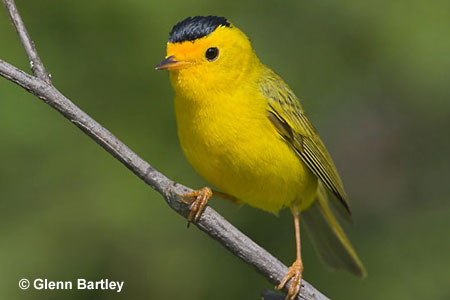
\includegraphics[width=0.65\textwidth]{pics/wilsons_warbler.jpeg}
\end{center}
\end{columns}


\end{frame}

%==================================================================================================

\section{Model}

\begin{frame}
\frametitle{Allele Frequency Model}

For the allele $i$, from locus $l$, at location $k$


\[ \bm{y_{l \cdot k}} \sim \text{Multinomial}\left(n_{lk},\: \bm{f}_{l \cdot k}\right) \quad n_{lk}=\textstyle\sum_i y_{lik}\]
\[ f_{lik} = \frac{\exp(\Theta_{lik})}{\sum_i \exp(\Theta_{lik})} \quad
\bm{\Theta}_{li} \sim \mathcal{N}( \bm{M}_{li}, \bm{\Sigma_{}})
\]

\pause

Posterior:
\begin{align*}
       &~\prod_l \prod_k \frac{n_{lk}!}{\prod_i y_{lik}!} \textstyle\prod_i \left( \frac{\exp(\Theta_{lik})}{\sum_i \exp(\Theta_{lik})} \right)^{y_{lik}} \\
\times &~\prod_l \prod_i 2\pi^{-r/2} |\bm\Sigma|^{-1/2} \exp\left[ -\frac{1}{2}(\bm{\Theta}_{li} - \bm{M}_{li})'\bm\Sigma^{-1} (\bm{\Theta}_{li} - \bm{M}_{li}) \right]\\
\times &~\pi(\bm{M}, \bm{\Sigma})
\end{align*}

\end{frame}

%==================================================================================================

\begin{frame}
\frametitle{Model Output}

\only<1>{
\begin{center}
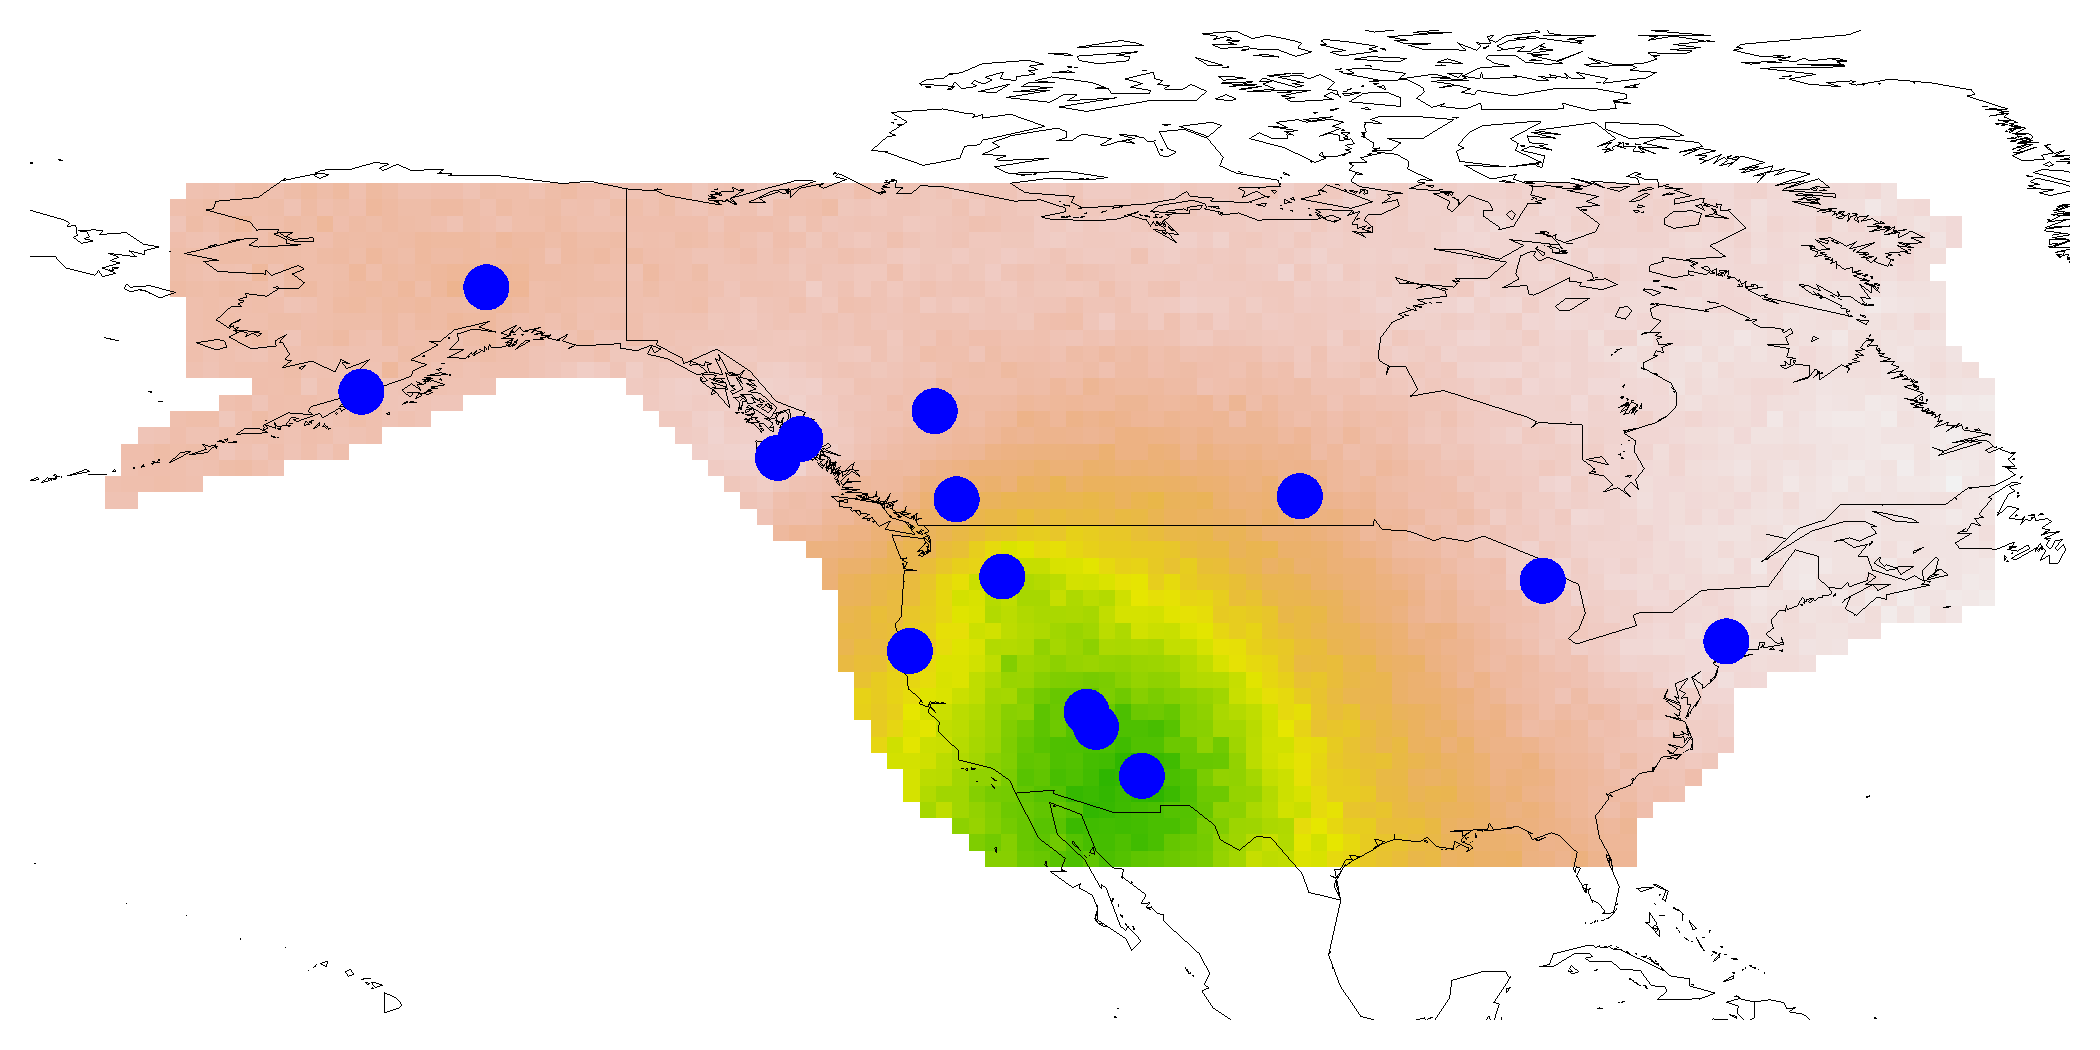
\includegraphics[width=0.9\textwidth]{pics/HETH_Al3-1.pdf}
\end{center}
}

\only<2>{
\begin{center}
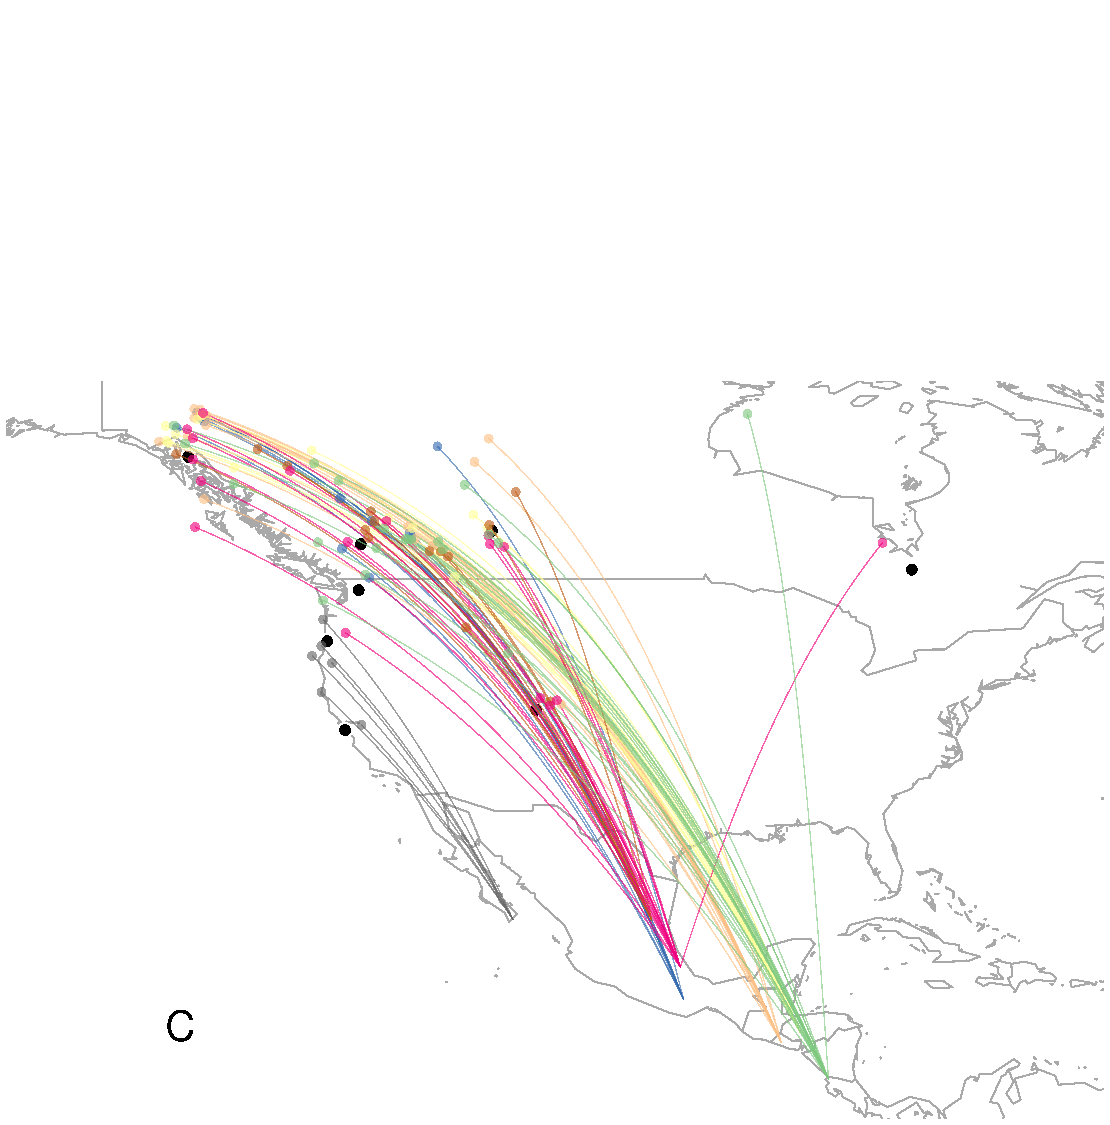
\includegraphics[width=0.9\textwidth]{pics/connectivity.pdf}
\end{center}
}

\end{frame}

%==================================================================================================

\begin{frame}
\frametitle{Implementation}

Model fitting and prediction is done via MCMC \\
\begin{itemize} \addtolength{\itemsep}{3mm}
\item Original implementation in pure C++ with minimal dependencies (Wasser, et al. (2004))
\item Rewritten using R / C++ via Rcpp(Armadillo) 
\begin{itemize}
\item Code closer to matrix notation (and R)
\item Transparent use of high performance LAPACK implementations (ATLAS, OpenBLAS, Intel MKL)
\end{itemize}
\item GPU based optimizations were added using CUDA, CUBLAS, and MAGMA libraries
\item R package isoscatR (available on Github now, CRAN soon)
\end{itemize}

\end{frame}


%==================================================================================================
%==================================================================================================

\begin{frame}
\frametitle{Performance}

{\small System specs - 4 core Intel i5-2500K, GeForce GTX 460} \\
{\small Software specs - Ubuntu 13.04, OpenBlas 0.2.6, CUDA 5.5 RC, Magma 1.4 beta1} \\
~\\
\pause

Performance during model fitting is quite good ... \\

\begin{center}
300,000 iterations in $\sim 5.5$ minutes
\end{center}

\pause 

Performance during prediction is much slower ... \\
\begin{center}
1,000 prediction iterations in $\sim 30$ mins \\
(predictions calculated every 100 iterations)
\end{center}

\pause

Not too bad in the greater scheme of things, but we need to perform cross validation ($150-200$ runs per species) ...

\end{frame}

%==================================================================================================

\begin{frame}
\frametitle{Prediction details}

Why is the prediction slow? \pause Predicting allele frequencies for Hermit thrush at 3318 novel locations.\\
~\\
To do so we sample from:
\[ \bm{\Theta}_p | \bm{\Theta}_m \sim \mathcal{N}(\bm{\mu}_p+\bm\Sigma_{pm}\bm\Sigma_{m}^{-1}(\bm{\Theta}_m-\bm\mu_m),\: \bm\Sigma_{p}-\bm\Sigma_{pm}\bm\Sigma_{m}^{-1}\bm\Sigma_{mp}) \]

\pause

\vspace{-3mm}

\begin{columns}
\column{0.20\textwidth}
\column{0.60\textwidth}
\begin{block}{Algorithm steps}
\begin{enumerate}
\item Calculate $\bm\Sigma_{pm}$ and $\bm\Sigma_{p}$
\item Calculate $\text{Chol}(\bm\Sigma_{p}-\bm\Sigma_{pm}\bm\Sigma_{m}^{-1}\bm\Sigma_{mp})$
\item Sample from MVN
\item Calculate allele frequencies
\item Output results
\end{enumerate}
\end{block}
\column{0.2\textwidth}
\end{columns}
\end{frame}

%==================================================================================================

\begin{frame}
\frametitle{Prediction algorithm timings}

\vfill

\begin{center}

\begin{tabular}{rl|c|c|c|}
\hline
& Step                                    & CPU (secs)  & CPU+GPU (secs)  & Rel. Improvement \\
\hline
1. & Covariances                          & 1.080       & \only<2>{0.046} & \only<2>{23 } \\
2. & Cholesky                             & 0.467       & \only<2>{0.208} & \only<2>{2.3} \\
3. & Sample MVN                           & 0.049       & \only<2>{0.052} & \only<2>{0.9} \\
4. & Allele Freq                          & 0.129       & \only<2>{0.127} & \only<2>{1.0} \\
5. & Write                                & 0.007       & \only<2>{0.032} & \only<2>{0.2} \\
\hline 
   & Total                                & 1.732       & \only<2>{0.465} & \only<2>{3.7} \\
\end{tabular}

\end{center}

\vfill

\end{frame}


% Performance (CPU) :
% =============================================
% Step 1: 1.08 (0.0106)
% Step 2: 0.000174 (5.15e-06)
% Step 3: 0.467 (0.00171)
% Step 4: 0.0491 (0.000725)
% Step 5: 0.129 (0.000273)
% Step 6: 0.00654 (0.0338)


% Performance (CPU+GPU) :
% =============================================
% Step 1: 0.0462 (0.000196)
% Step 2: 3.43e-05 (3.02e-06)
% Step 3: 0.208 (0.000229)
% Step 4: 0.0525 (0.000227)
% Step 5: 0.127 (0.00188)
% Step 6: 0.032 (0.231)


%==================================================================================================

\begin{frame}
\frametitle{Improving the Cholesky step}

Not surprising given Cholesky factorization is $\mathcal{O}(n^3)$ and $n=3318$.\\
~\\
There isn't a magical solution to this, so we just want to use the fastest possible implementation of the Cholesky decomposition.

\begin{itemize}
\item \textbf{Intel MKL / ATLAS / Eigen} - all (multicore) CPU based with very marginal improvement 
\item \textbf{CUBLAS} - part of NVidia's CUDA toolkit, implements core BLAS functions (but not Cholesky) 
\item \textbf{CULA} - proprietary / closed source (dense and sparse) GPU linear algebra library with an expensive license
\item \textbf{MAGMA} - open source Multicore+GPU dense hybrid linear algebra library (CUDA and OpenCL implementations)
\end{itemize}

\end{frame}

%==================================================================================================

\begin{frame}
\frametitle{Cholesky GPU}

\vfill
\begin{center}
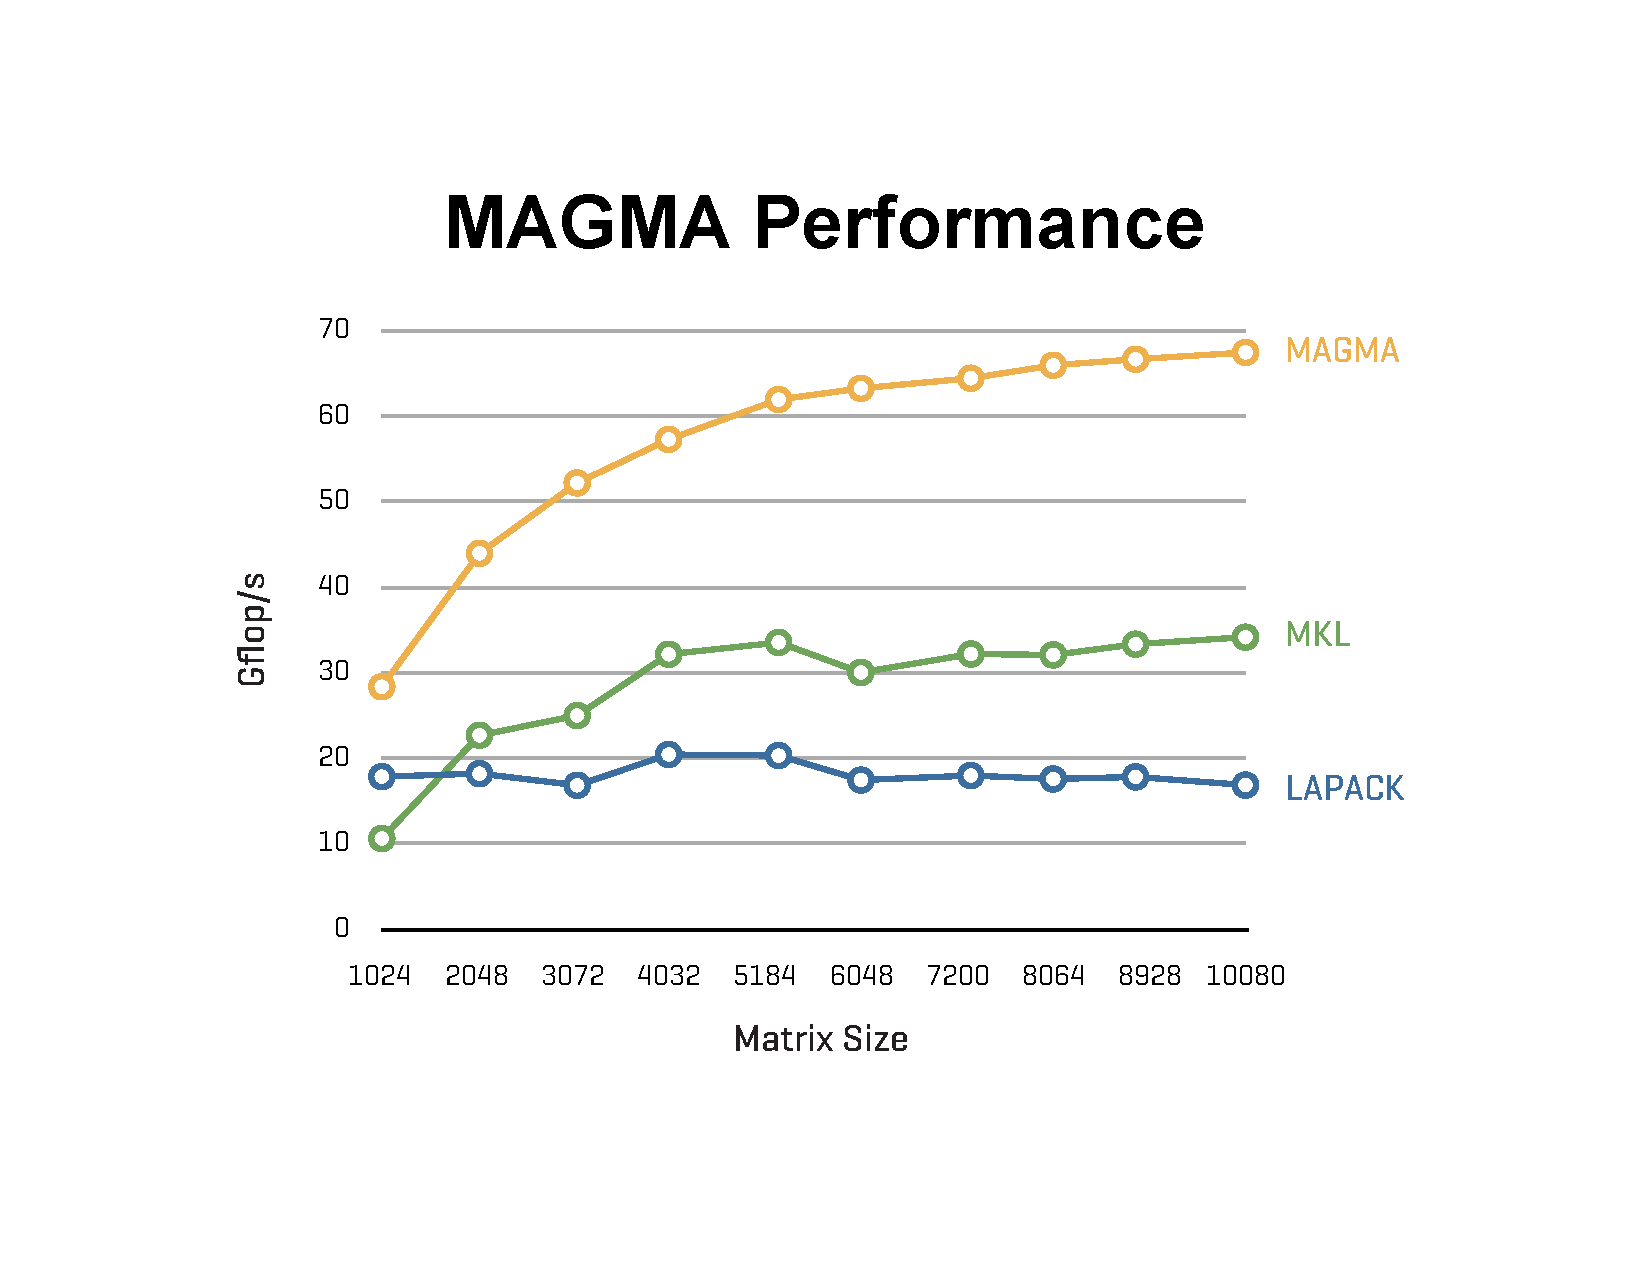
\includegraphics[width=0.7\textwidth]{pics/magma_chol.pdf}
\end{center}
\vfill
{\tiny Ltaief, H. ``A Scalable High Performant Cholesky Factorization for Multicore with GPU Accelerators''\\ VECTAR'10 Presentation, Berkeley, CA, June 22-25, 2010.}
\end{frame}

%==================================================================================================

\begin{frame}[fragile]
\frametitle{Additional Considerations}

\begin{itemize}
\item There are costs for moving data on to and off of the GPU
\item Once the data is there, may as well do as many calculations as possible
\begin{itemize}
\item Drawing sample from the GP is sped up by performing the matrix multiplication on the GPU
\end{itemize}
\item GPU code is much more verbose / dense (calculating $\bm\Sigma_{pm}\bm\Sigma_{m}^{-1}$)
\end{itemize}

\pause

{\scriptsize
\begin{columns}
\column{0.0125\textwidth}
\column{0.45\textwidth}
\begin{block}{Armadillo}
\begin{minted}{c++}
arma::mat tmp = cov12.t() * p.Sinv
\end{minted}
\end{block}
\column{0.025\textwidth}
\column{0.475\textwidth}
\begin{block}{GPU (CUBLAS)}
\begin{minted}{c++}
cublasDgemm_v2( 
    p.handle, CUBLAS_OP_T, CUBLAS_OP_N,
    n_pred, n_known, n_known,
   &one,
    p.d_cov12, n_known,
    p.d_invcov11, n_known,
   &zero,
    p.d_tmp, n_pred
)
\end{minted}
\end{block}
\column{0.0125\textwidth}
\end{columns}
}

\end{frame}

%==================================================================================================

\begin{frame}[fragile]
\frametitle{Improving Covariance calculations}

Covariance in our model is assumed to be stationary and isotropic (depends only on distance between locations)
\begin{itemize}
\item Elements of the covariance matrix can be calculated independently
\item Small scale ``embarrassingly parallel'' $\Rightarrow$ good candidate for the GPU.
\item Implementation is straight forward (if we ignore things like symmetry)
\end{itemize}


\pause

\begin{block}{}
{\scriptsize
\begin{minted}{c}
__global__ void powered_exponential_kernel(double* dist, double* cov,
                                           const int n, const int nm,
                                           const double sigma2, const double phi,
                                           const double kappa, const double nugget) 
{
    int n_threads = gridDim.x * blockDim.x;
    int pos = blockDim.x * blockIdx.x + threadIdx.x;

    for (int i = pos; i < nm; i += n_threads)
        cov[i] = sigma2 * exp(-pow(dist[i] / phi, kappa)) + nugget*(i%n == i/n);
}
\end{minted}
}
\end{block}

\end{frame}

%==================================================================================================

\begin{frame}
\frametitle{Summary}

Relatively small changes in one function resulted in $3-4$x improvement
\begin{itemize}
\item Cross validation results in a day or two and not a week
\item Started with trying to find an improved Cholesky decomposition, other optimizations followed
\item GPU implementation was relatively painless
\item Libraries are under active development (read: things can and will break)
\item External libraries make package development more complicated
\end{itemize}

\end{frame}

%==================================================================================================

\begin{frame}
\frametitle{What's next?}

Much of these details are specific to this particular problem, but the approach suggests common tasks/bottlenecks that turn up when working with Gaussian Processes.\\
~\\ \pause
To that end ...

\begin{itemize}
\item Later this summer - hopefully releasing RcppGP package
\begin{itemize}
\item Talk at JSM 2013 in Montreal
\end{itemize}
\item Low level CPU and GPU R and C++ utility functions 
\item Methodology agnostic
\item Support for composite covariance functions
\end{itemize}

\pause

\begin{center}
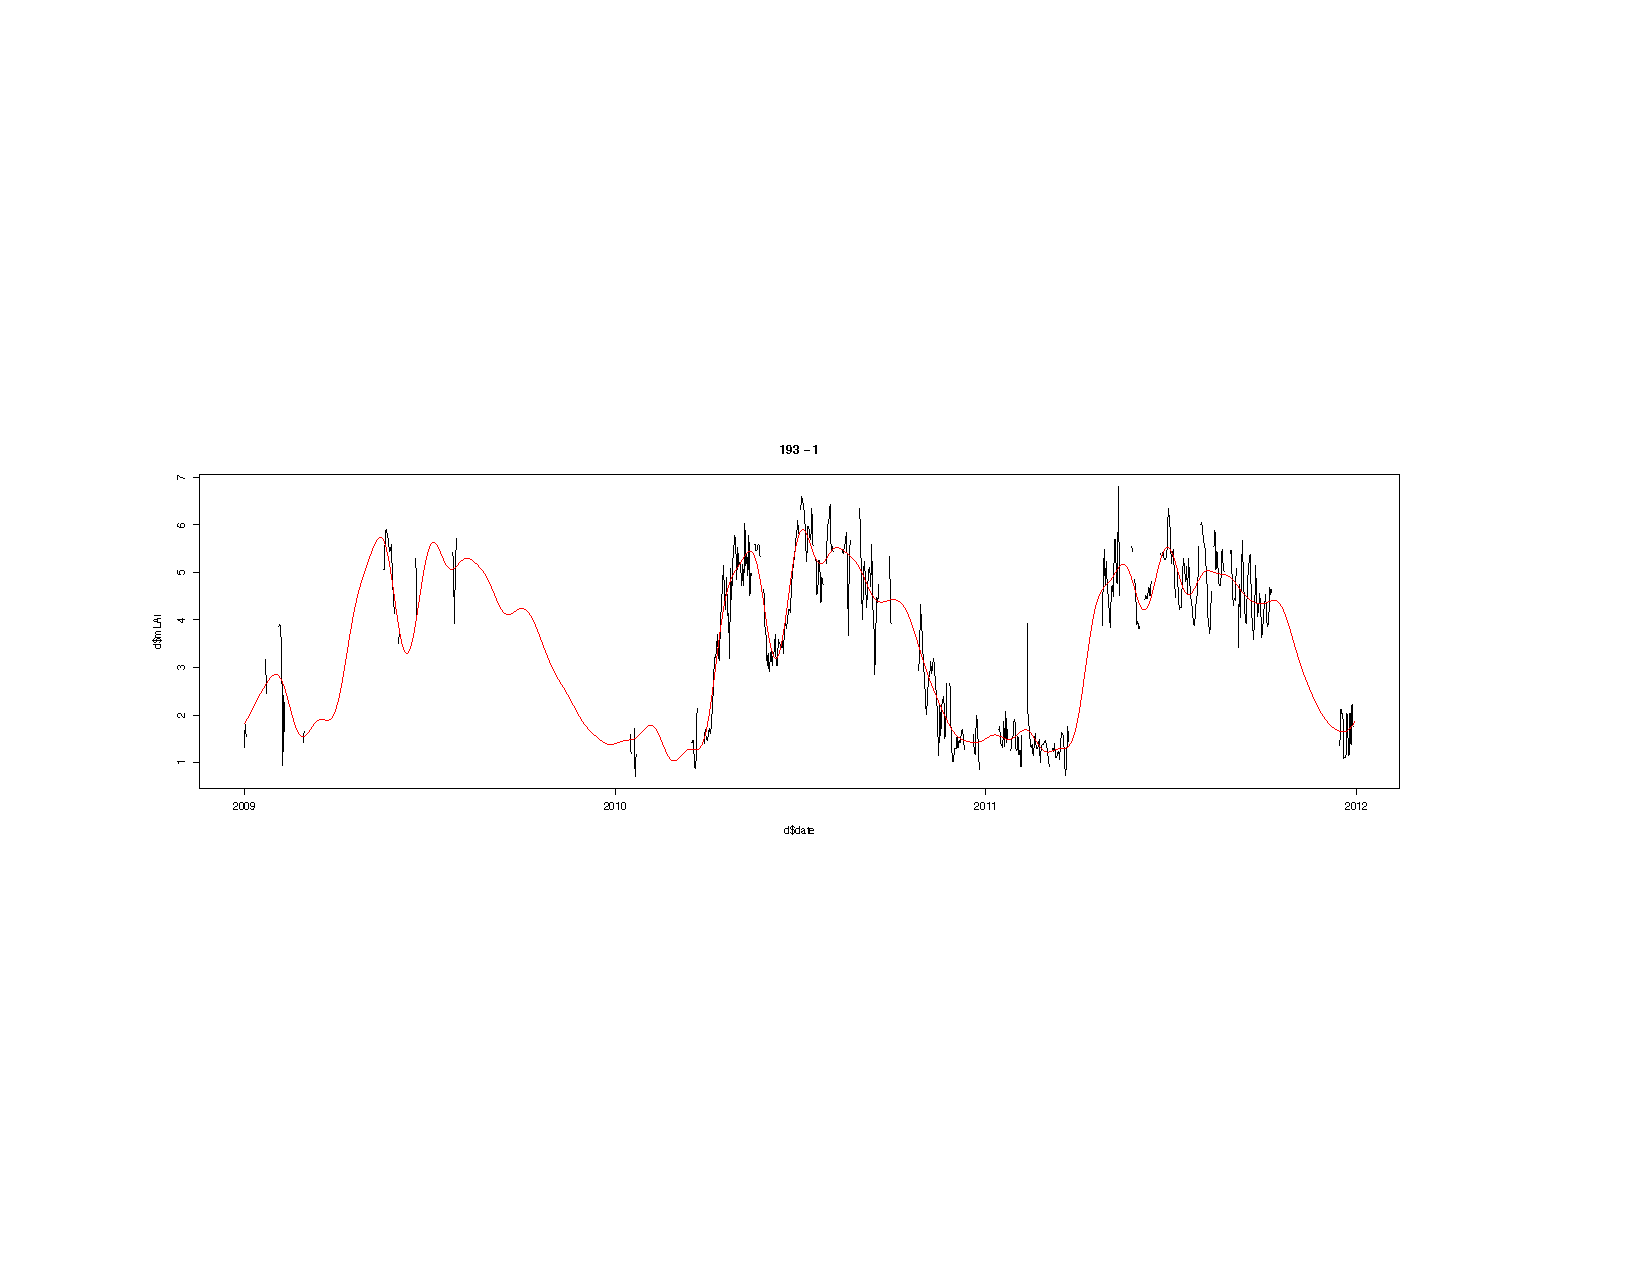
\includegraphics[width=0.9\textwidth]{pics/sensor.pdf}
\end{center}

\end{frame}

%==================================================================================================


\begin{frame}
\frametitle{Questions, Comments?}
\vfill
\begin{center}
{\Large
\renewcommand*\arraystretch{1.5}
\begin{tabular}{lll}
email        & : & rundel@gmail.com \\
github       & : & {\normalsize \urlwofont{http://github.com/rundel/}} \\
presentation & : & {\normalsize \urlwofont{http://github.com/rundel/Presentations/}} \\
\end{tabular}
}
\end{center}
\vfill
\end{frame}


%\section{Supplementary}
%
%\begin{frame}
%\only<1>{
%\frametitle{Sampling Locations (Hermit Thrush)}
%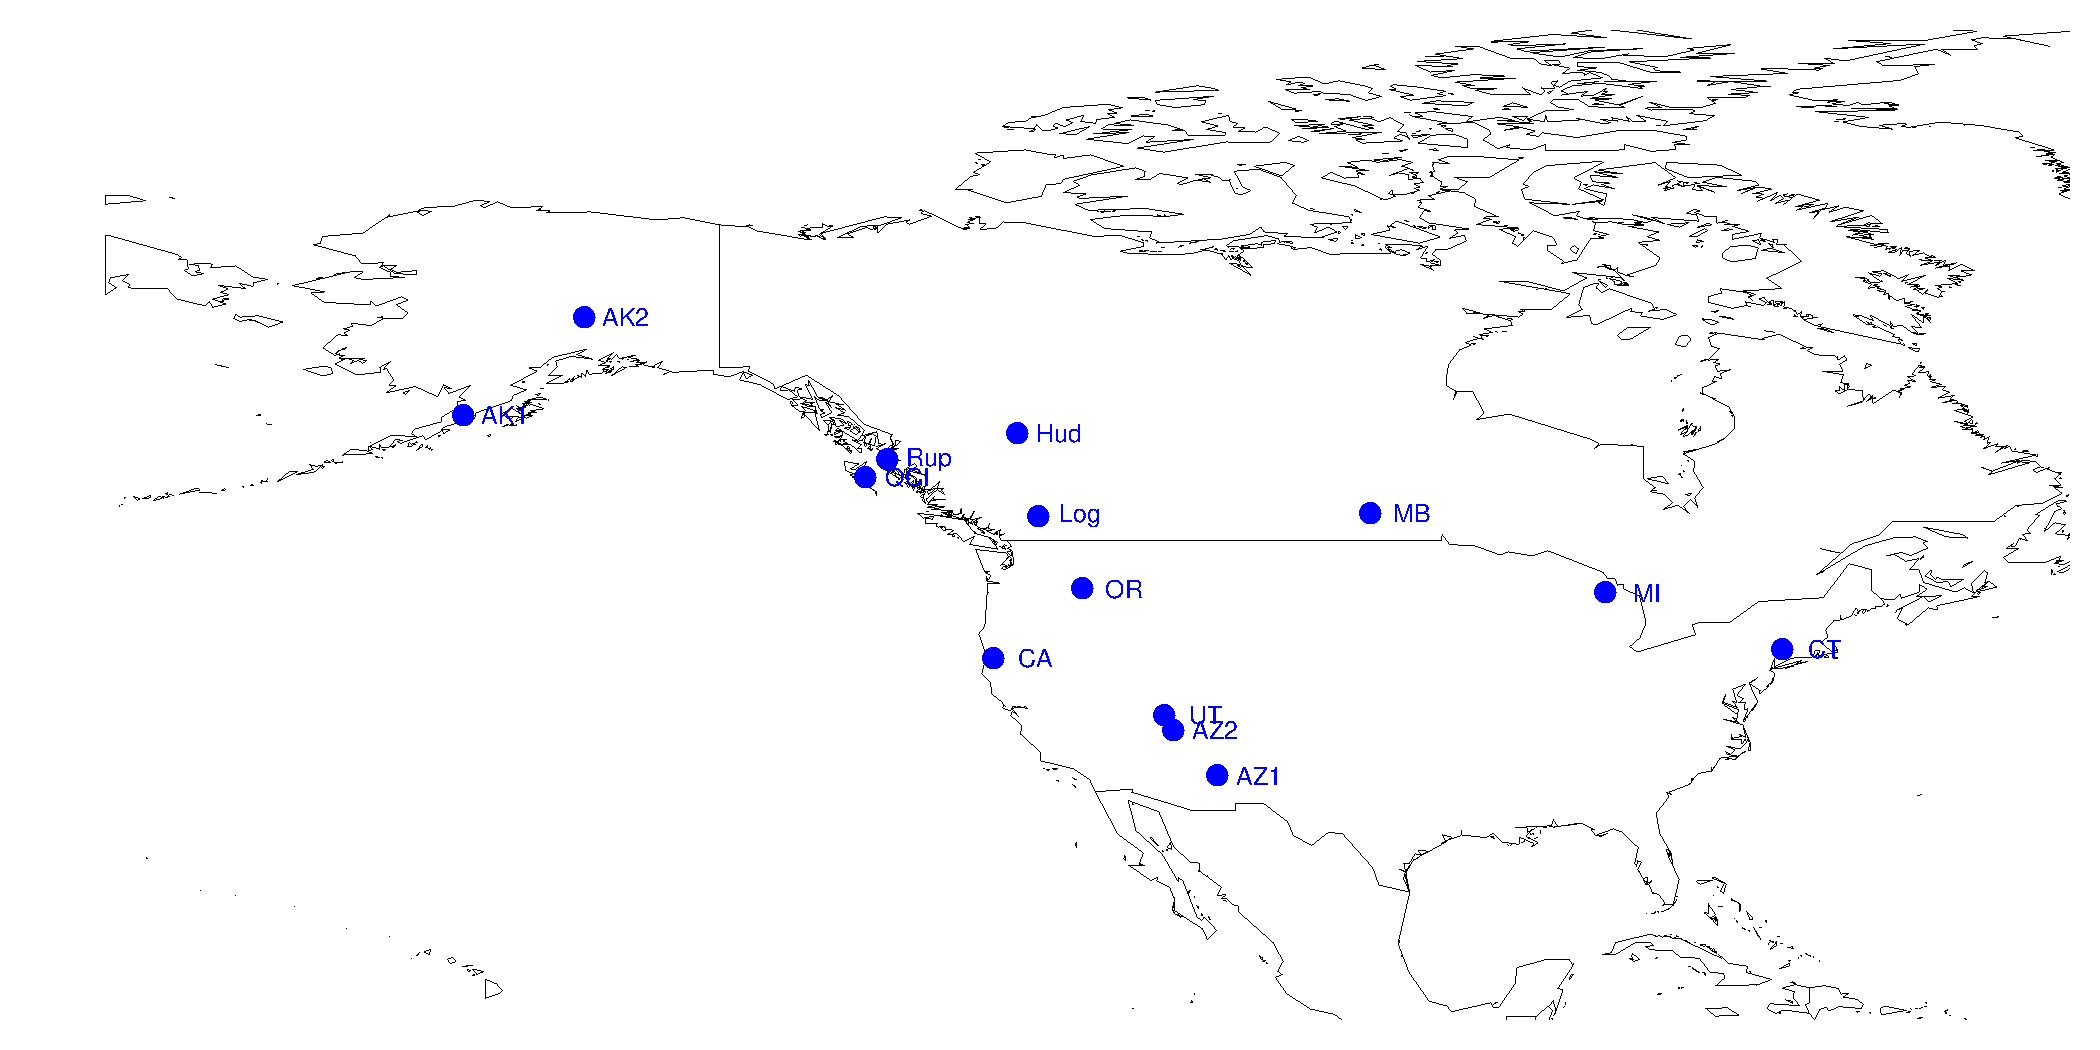
\includegraphics[width=\textwidth]{pics/HETH_locs.pdf}
%}
%\only<2>{
%\frametitle{Sampling Locations (Wilson's Warbler)}
%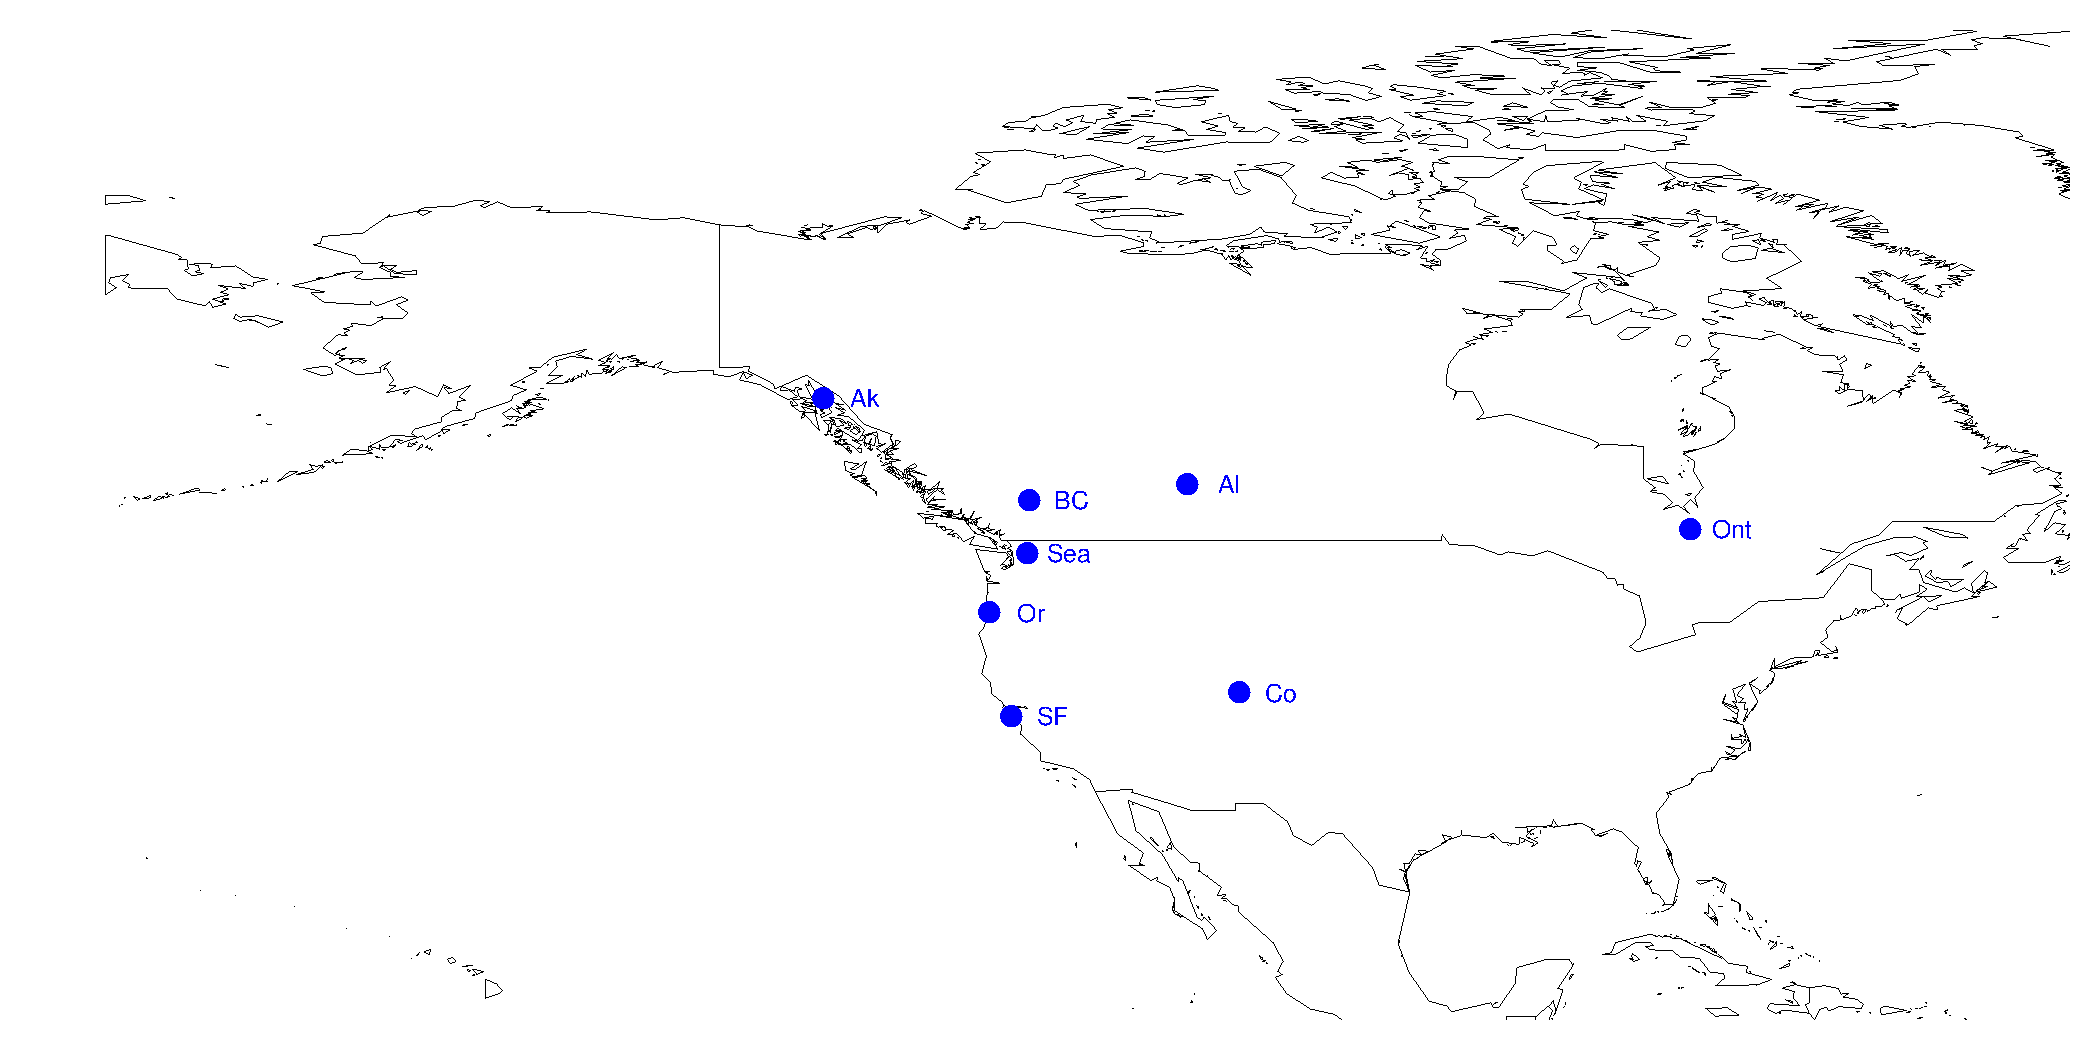
\includegraphics[width=\textwidth]{pics/WIWA_locs.pdf}\\
%}
%\end{frame}

\end{document}